In this section, using the continuous-time DCDP framework, we develop the social planner's problem. When an opportunity to drill potential well sites arrives, the social planner makes two decisions. First, the planner must choose, via the choice of $Pr_{t}$, the aggregate quantity of drilling. Second, the planner must also decide which locations will be drilled. Each site can be indexed by $\epsilon_{1t} - \epsilon_{0t}$, and so selecting which sites to drill can be thought of as selecting which indices to drill. Because there is a continuum of potential well locations, determining the optimal policy (i.e., the optimal $Pr_{t})$ is simply to choose a threshold that does not depend on the specific set of cost shocks realized at time $t$. Potential well locations with indices above the threshold drill, whereas those below it wait to drill. The one-to-one mapping between the threshold index and the choice of $Pr_{t}$ is characterized by equation (\ref{Equation:DCDP-Model_Decision-Rule}).

The goal of the social planner is to maximize welfare in the market. In this maximization problem, for a given $Pr_{t}$, the market's welfare obtained from potential well sites at time $t$ is defined as follows\footnote{Using $D_{t}$, we can re-write the definition: $W_{t}^{sp} \ = \ R_{t} f_{t} \ + \ u(\alpha D_{t}) \ - \ c(D_{t}) \ + \ D_{t} \sigma \big( \gamma \ - \ \ln(Pr_{t}) \big) \ + \ (\lambda_{a} R_{t} - D_{t}) \sigma \big( \gamma \ - \ \ln(1 - Pr_{t}) \big)$.}:
\begin{equation}
\begin{split}
     W_{t}^{sp} \ 
     & \equiv \ R_{t} f_{t} \\
     & \hspace{0.7cm} + \ u(\alpha \lambda_{a} R_{t} Pr_{t}) \ - \ c(\lambda_{a} R_{t} Pr_{t}) \\
     & \hspace{0.7cm} + \ \lambda_{a} R_{t} \Big\{ Pr_{t} \cdot \sigma \big( \gamma \ - \ \ln(Pr_{t}) \big) \ + \ (1 - Pr_{t}) \cdot \sigma \big( \gamma \ - \ \ln(1 - Pr_{t}) \big) \Big\}
\label{Equation:Social-Planners-Problem_Welfare}
\end{split}
\end{equation}
As shown, the welfare of the market at time $t$ consists of three components.\footnote{$W_{t}^{sp}$ can be interpreted differently. To be specific, $W_{t}^{sp}$ is the sum of the flow payoff from the undrilled well sites at time $t$ $\left( \text{i.e., } R_{t} f_{t} \right)$, the net (expected) payoff obtained from the marginally drilled well site at time $t$ $\left( \text{i.e., } u(\alpha \lambda_{a} R_{t} Pr_{t}) - c(\lambda_{a} R_{t} Pr_{t}) + \lambda_{a} R_{t} Pr_{t} \sigma \big( \gamma \ - \ \ln(Pr_{t}) \big) \right)$, and the (expected) gains from the well sites that are available but decided not to drill at time $t$ $\left( \text{i.e., } \lambda_{a} R_{t} (1 - Pr_{t}) \sigma \big( \gamma \ - \ \ln(1 - Pr_{t}) \big) \right)$.} The first line indicates the flow payoff received from undrilled well locations at time $t$. The second line means the choice-specific instantaneous payoff, which is presented as equation (\ref{Equation:DCDP-Model_Payoff-Function_Social-Planners-Problem}). The last line suggests the payoff related to choice-specific cost shocks.\footnote{The last line in equation (\ref{Equation:Social-Planners-Problem_Welfare}) can be rewritten using $e_{0}$ and $e_{1}$: \par \hspace{0.3cm} $\lambda_{a} R_{t} \big\{ Pr_{t} \cdot \sigma \big( \gamma \ - \ \ln(Pr_{t}) \big) \ + \ (1 - Pr_{t}) \cdot \sigma \big( \gamma \ - \ \ln(1 - Pr_{t}) \big) \big\} \ = \ \lambda_{a} R_{t} \big\{ Pr_{t} \cdot e_{1} \ + \ (1 - Pr_{t}) \cdot e_{0} \big\}$.} Note that regarding the choice-dependent cost shocks, their expected value is used and that only the terms in the last two lines, which depend on the social planner's drilling decisions, are associated with $\lambda_{a}$. 

In the continuous-time DCDP framework, the social planner's welfare problem is given by
\begin{footnotesize}
\begin{equation}
\begin{split}
     \underset{\{Pr_{t}\}_{t = 0}^{\infty}}{\max} \hspace{0.1cm} \int_{0}^{\infty} e^{-rt} \bigg[ u(\alpha R_{t} Pr_{t}) - c(R_{t} Pr_{t}) + R_{t} f_{t} + R_{t} \Big\{ Pr_{t} \cdot \sigma \big( \gamma - \ln(Pr_{t}) \big) + (1 - Pr_{t}) \cdot \sigma \big( \gamma - \ln(1 - Pr_{t}) \big) \Big\} \bigg] dt
\end{split}
\label{Equation:Social-Planners-Problem_Formulation}
\end{equation}
\end{footnotesize}
subject to
\begin{equation}
\begin{split}
    \dot{R}_{t} \ = \ -R_{t}Pr_{t} \ + \ E, \hspace{0.3cm} R_{0} \ = \ R(0) \ = \ 1 \hspace{0.2cm} \text{given,}
\end{split}
\label{Equation:Social-Planners-Problem_Law-of-Motion}
\end{equation}
\begin{equation}
\begin{split}
    R_{t} \ \geq \ 0, \hspace{0.3cm} 0 \ < \ Pr_{t} \ < \ 1.
\end{split}
\end{equation}
As shown, $W_{t}^{sp}$ is discounted at the rate of interest $r$. 

Under the assumption of an interior solution, the current-value Hamiltonian-Lagrangian of the social planner's problem is given by
\begin{equation}
\begin{split}
    \mathcal{H}^{sp} \ 
    & = \ R_{t} f_{t} \\
    & \hspace{0.7cm} + \ u(\alpha \lambda_{a} R_{t} Pr_{t}) \ - \ c(\lambda_{a} R_{t} Pr_{t}) \\
    & \hspace{0.7cm} + \ \lambda_{a} R_{t} \big\{ Pr_{t} \cdot \sigma \big( \gamma \ - \ \ln(Pr_{t}) \big) \ + \ (1 - Pr_{t}) \cdot \sigma \big( \gamma \ - \ \ln( 1 - Pr_{t}) \big) \big\} \\
    & \hspace{0.7cm} + \ \pi_{t} (-\lambda_{a} R_{t} Pr_{t} + E).
%    \ + \ \lambda_{1,t} (R_{t}) \ + \ \lambda_{2,t} (1 - Pr_{t}) \ + \ \lambda_{3,t} (Pr_{t}).
\end{split}
\label{Equation:Social-Planners-Problem_Hamiltonian-Lagrangian}
\end{equation}

The necessary conditions of the current-value Hamiltonian-Lagrangian are as follows:
\begin{equation}
\begin{split}
    & R_{t} \big\{ \alpha u'(\alpha R_{t} Pr_{t}) \ - \ c'(R_{t} Pr_{t}) \ - \ \sigma \ln(Pr_{t}) \ + \ \sigma \ln(1 - Pr_{t}) \ - \ \pi_{t} \big\} \ \leq \ 0, \hspace{0.2cm} Pr_{t} \ \geq \ 0,  \hspace{0.2cm} \text{C.S.}, \\
%    \ - \ \lambda_{2,t} \ + \ \lambda_{3,t} \ \leq \ 0, \\
%    & \hspace{0.5cm} Pr_{t} \ \geq \ 0,  \hspace{0.2cm} \text{C.S.},
\end{split}
\label{Equation:Social-Planners-Problem_Necessary-Conditions_Drilling-Probability}
\end{equation}
\begin{equation}
\begin{split}
    \dot{\pi}_{t} \ 
    & = \ r \pi_{t} \ - \ \left\{ f_{t} \ + \ \sigma \big( \gamma \ - \ \ln(1 - Pr_{t}) \big) \right\},
%     \ - \ \lambda_{1,t},
\end{split}
\label{Equation:Social-Planners-Problem_Necessary-Conditions_Costate-Variable}
\end{equation}
\begin{equation}
\begin{split}
    \lim_{t \rightarrow \infty} e^{-rt} (R_{t} \pi_{t}) \ = \ 0.
\end{split}
\label{Equation:Social-Planners-Problem_Transversality-Condition}
\end{equation}
If $R_{t} > 0$, necessary condition (\ref{Equation:Social-Planners-Problem_Necessary-Conditions_Drilling-Probability}) yields the following expression for the costate variable $\pi_{t}$, which is a function of $R_{t}$ and $Pr_{t}$:
\begin{equation}
\begin{split}
    \pi_{t} \ 
    & = \ \alpha u'(\alpha R_{t} Pr_{t}) \ - \ c'(R_{t} Pr_{t}) \ - \ \sigma \ln(Pr_{t}) \ + \ \sigma \ln(1 - Pr_{t}) \\
    & = \ \big\{ \alpha u'(\alpha R_{t} Pr_{t}) \ - \ c'(R_{t} Pr_{t}) \ + \ \sigma \big( \gamma \ - \ \ln(Pr_{t}) \big) \big\} \ - \ \sigma \big( \gamma \ - \ \ln(1 - Pr_{t}) \big).
\end{split}
\label{Equation:Social-Planners-Problem_Meaning-of-Costate-Variable}
\end{equation}
In addition, substituting condition (\ref{Equation:Social-Planners-Problem_Meaning-of-Costate-Variable}) into condition (\ref{Equation:Social-Planners-Problem_Necessary-Conditions_Costate-Variable}) yields the following Euler equation that governs the dynamics of the social planner's welfare maximization problem over time:
\begin{equation}
\begin{split}
    % \dot{\pi}_{t} \ 
    % & = \ r \pi_{t} \ - \ \sigma \big( \gamma \ + \  \ln(1 - Pr_{t}) \big) \\
    % (\dot{\pi}_{t} \ - \ r\pi_{t}) e^{-rt} \
    % & = \ - \sigma \big( \gamma \ - \ \ln(1 - Pr_{t}) \big) e^{-rt} \\
    % \pi_{t} e^{-rt} \
    % & = \ \int_{t}^{\infty} e^{-r\tau} \sigma \big( \gamma \ - \ \ln(1 - Pr_{\tau}) \big) d\tau \ + \ \mathcal{C} \\  % C = 0 from the equation for \pi_{t} at the steady state.
    \pi_{t} \
    & = \ e^{rt} \left[ \int_{t}^{\infty} e^{-r\tau} \Big\{ f_{t} \ + \ \sigma \big( \gamma \ - \ \ln(1 - Pr_{\tau}) \big) \Big\} d\tau \right],
\end{split}
\label{Equation:Social-Planners-Problem_Euler-Equation}
\end{equation}
We will discuss the implications of necessary conditions (\ref{Equation:Social-Planners-Problem_Necessary-Conditions_Costate-Variable}) and (\ref{Equation:Social-Planners-Problem_Meaning-of-Costate-Variable}) later. 

The social planner's problem has a unique steady state $(R_{ss}, \pi_{ss})$ such that $\dot{R}_{ss}, \ \dot{\pi}_{ss} = 0$. From necessary conditions (\ref{Equation:Social-Planners-Problem_Law-of-Motion}) and (\ref{Equation:Social-Planners-Problem_Necessary-Conditions_Costate-Variable}), $R_{t}$ and $\pi_{t}$ must satisfy the following equations at steady state:
\begin{equation}
    \begin{cases}
        \begin{split}
        \ R_{ss} \
        & = \ \frac{E}{ \ \lambda_{a} Pr_{ss} \ } \\
        \ \pi_{ss} \
        & = \ \frac{ \ f_{t} \ + \ \lambda_{a} \sigma \left( \gamma \ - \ \ln(1 - Pr_{ss}) \right) \ }{r}.
        \end{split}
    \end{cases}
\label{Equation:Social-Planners-Problem_System-of-Equations-for-Steady-State}
\end{equation}
On top of the equations, necessary condition (\ref{Equation:Social-Planners-Problem_Meaning-of-Costate-Variable}) has to hold at the steady state simultaneously. Solving the system of three equations, we can uniquely identify $(R_{ss}, \pi_{ss})$, including the value of the control variable at the steady state (i.e., $Pr_{ss}$). As implied by the first equation in (\ref{Equation:Social-Planners-Problem_System-of-Equations-for-Steady-State}), $R_{ss}$ is non-zero positive if $E \neq 0$. Using a Taylor series approximation, $\dot{R}_{t}$ and $\dot{\pi}_{t}$ can be linearized near the steady state $(R_{ss}, \pi_{ss})$, and this linearization process shows that the steady state of the infinite-horizon maximization problem is a saddle point, which is demonstrated in Figure \ref{Figure:Phase-Diagram_Saddle-Point}.\footnote{Regarding the saddle property, see \textit{9.5 Steady states in autonomous infinite-horizon problems} in \cite{Optimal-Control-Theory-and-Static-Optimization-in-Economics_Leonard-and-Long_1992}. And derivation details are provided in \ref{C3-Appendix_Derivations_Linearization-near-the-Steady-State-of-the-Social-Planners-Problem}.}
\afterpage{
    \begin{figure}[t!]
        \centering
        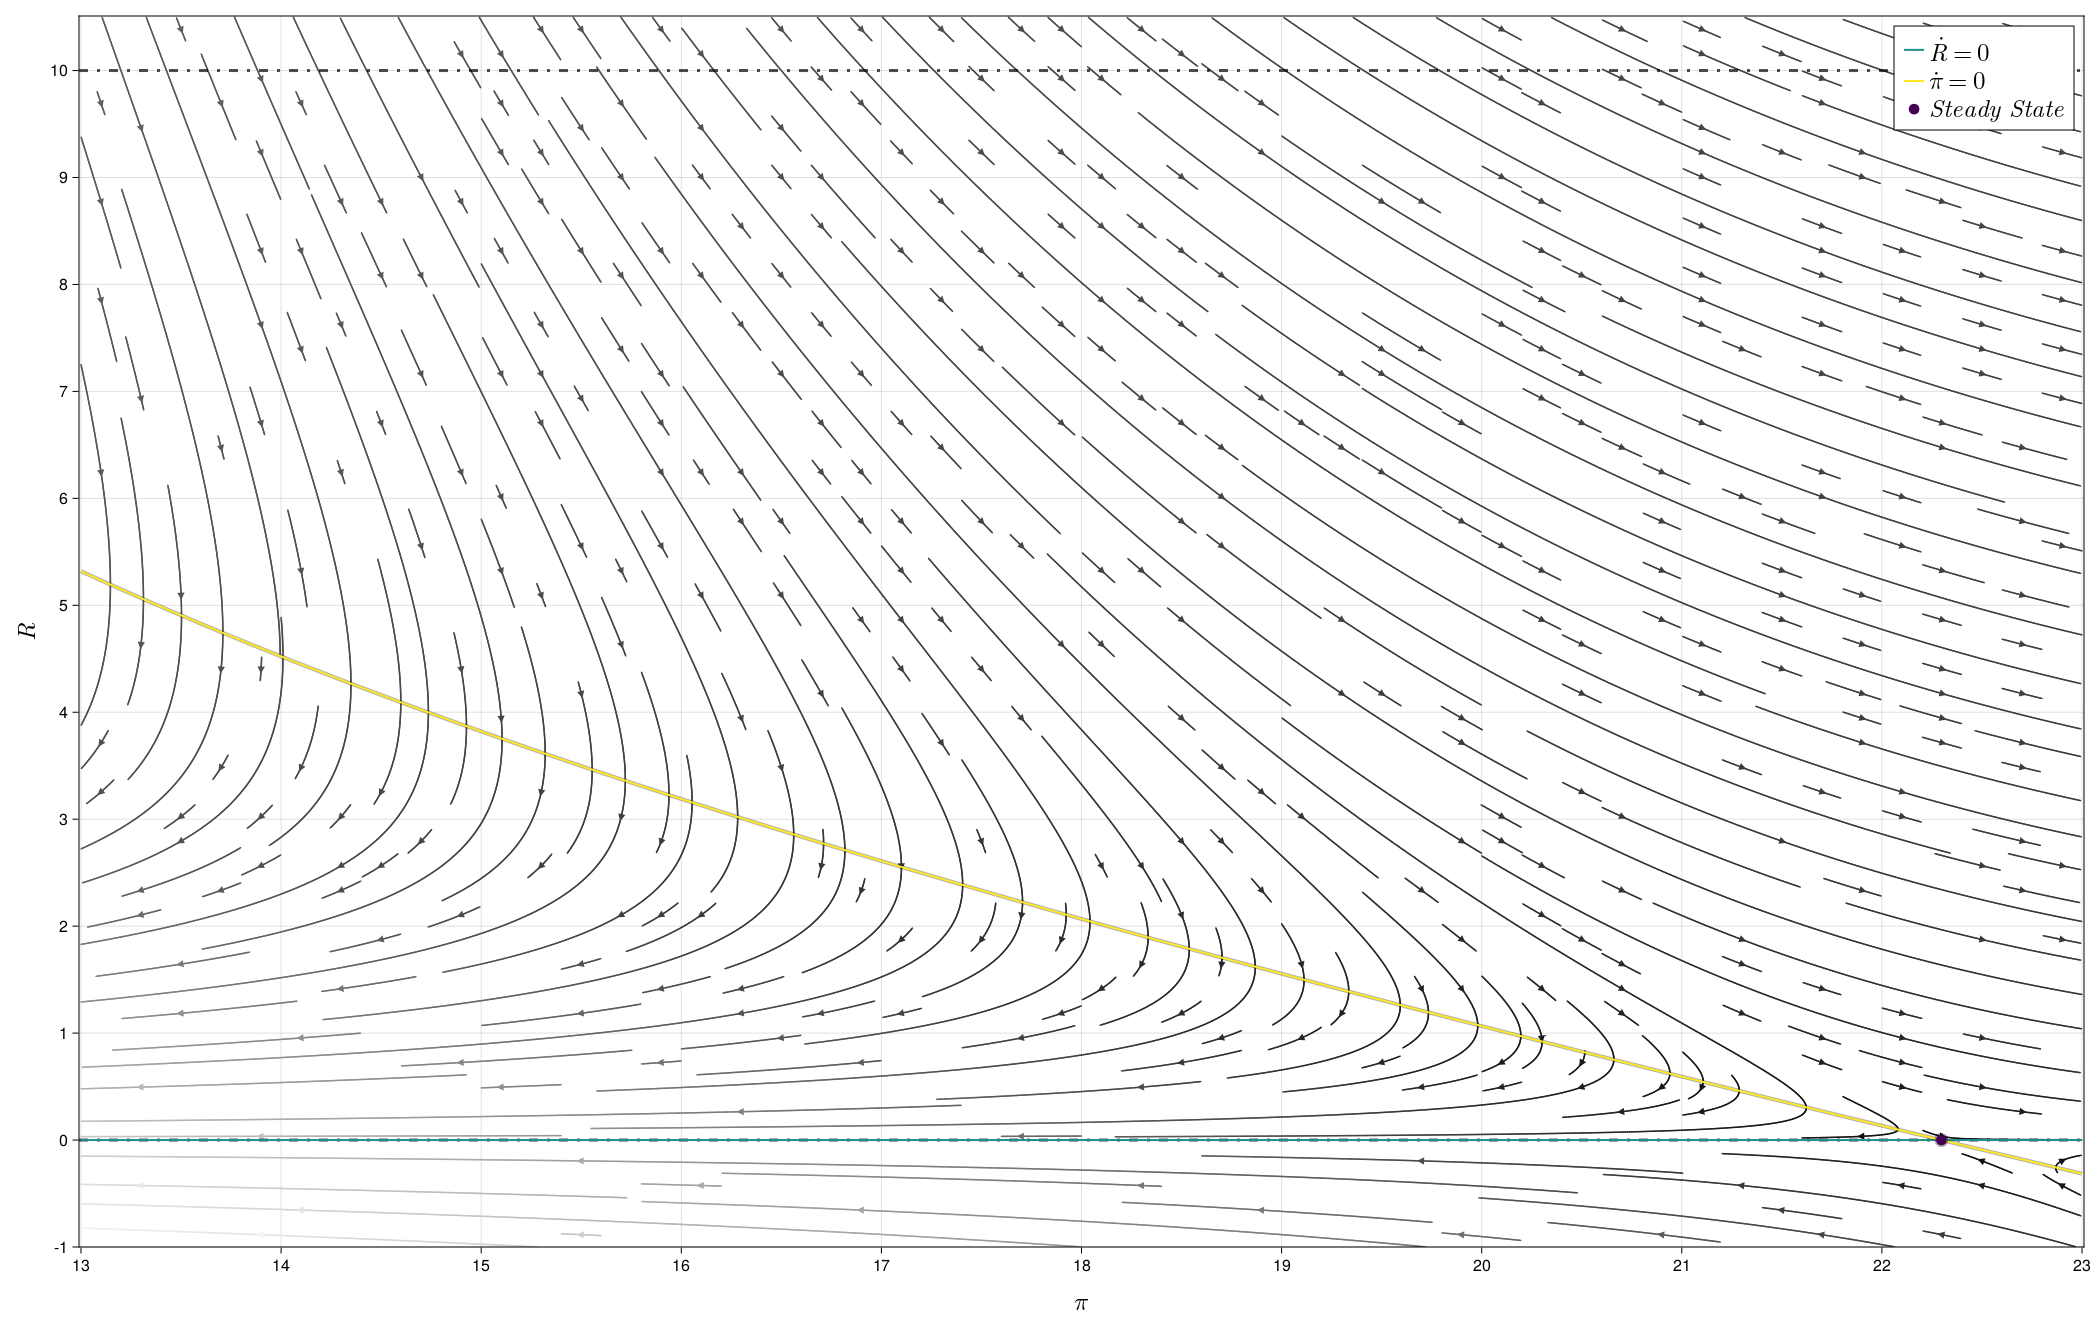
\includegraphics[scale = 0.195]{04_Chapter-3/00A_Figures/Figure_Equilibrium-Path_Endogenous-Price_Phase-Diagram_pi-by-R.png}
        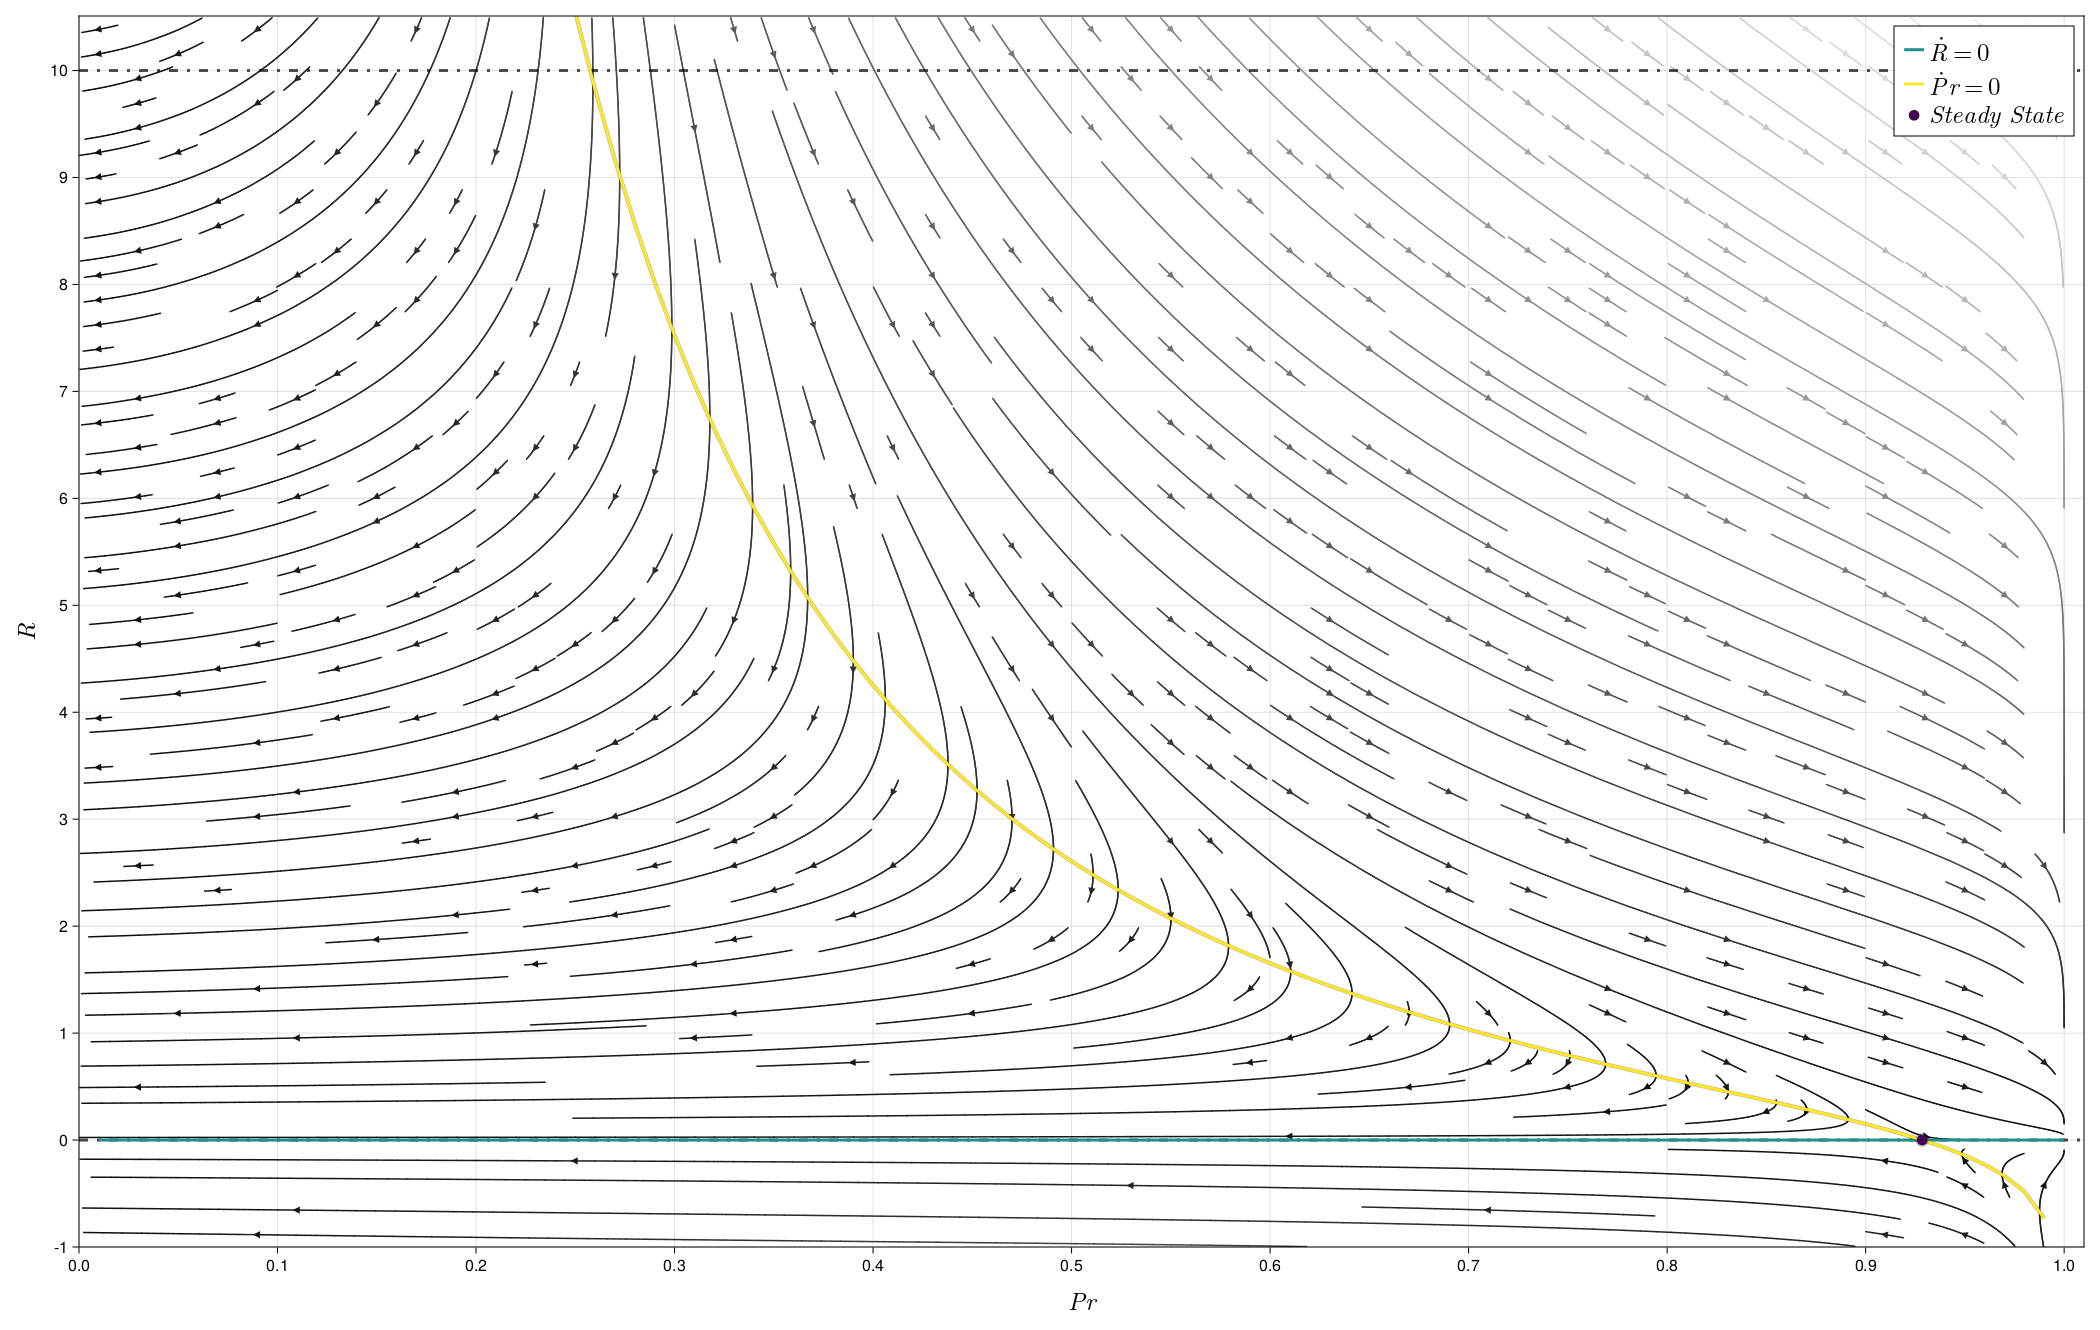
\includegraphics[scale = 0.195]{04_Chapter-3/00A_Figures/Figure_Equilibrium-Path_Endogenous-Price_Phase-Diagram_Pr-by-R.png}
        \caption{Phase Diagrams for the Social Planner's Problem}
        \caption*{
            {\small
            \textit{Note}: 
            This figure demonstrates two phase diagrams for the social planner's problem. The upper diagram illustrates that the steady state is exactly a saddle point. This figure assumes that a dispersion parameter of $\sigma = 1$, an interest rate of $r = 0.15$, an initial number of well sites of $R_{0} = 10$, additional well sites of $E = 0$, and exogenously given constant oil prices of $p = 50$. Also, a linear cost function of $c(D_{t}) = 2D_{t}$ is assumed.  
        }}
        \label{Figure:Phase-Diagram_Saddle-Point}
    \end{figure}
}
